\documentclass{standalone}
\usepackage{tikz}
\usetikzlibrary{positioning}
\usepackage{pgfplots}
\usepgfplotslibrary{groupplots}

\begin{document}
  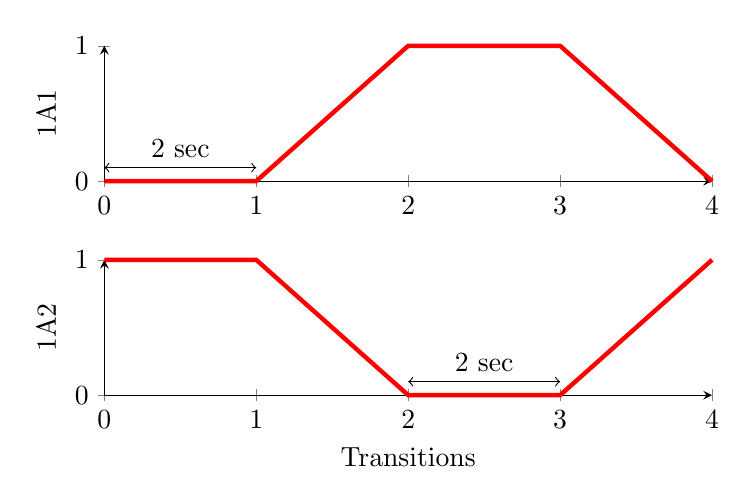
\begin{tikzpicture}
    \begin{groupplot} [
      group style={
        group name=timeplot,
        group size=1 by 2,
        xlabels at=all,
        horizontal sep=1cm,
        vertical sep=1cm,
      }, 
      clip=false,
      height=3.3cm, width=9.3cm,
      axis line style={->},
      axis lines=left,
      xlabel={},
      ylabel={},
      ytick={0,1},
      xtick={0,1,2,3,4},
      % grid=both,
      % xtick=\empty,
      % ytick=\XNOLL,
      % yticklabel=$x_0$,
      ]
      \nextgroupplot [ylabel={1A1},]
      \addplot[red, no marks,ultra thick,] coordinates {(0,0) (1,0) (2, 1) (3,1) (4, 0)};
      \draw[<->] (axis cs: 0, 0.1) -- node[above] {2 sec} (axis cs:1, 0.1);
      \nextgroupplot [ylabel={1A2}, xlabel={Transitions}]
      \addplot[red, no marks,ultra thick,] coordinates {(0,1) (1,1) (2, 0) (3,0) (4, 1)};
      \draw[<->] (axis cs: 2, 0.1) -- node[above] {2 sec} (axis cs:3, 0.1);
    \end{groupplot}
  \end{tikzpicture}
\end{document}
